\documentclass{article}
\usepackage[paper=letterpaper,margin=2cm]{geometry}
\usepackage[russian]{babel}
\usepackage[utf8]{inputenc}
\usepackage[]{graphicx}
\usepackage[usenames]{color}
\usepackage{colortbl}
\usepackage{geometry}
\usepackage{xcolor}
\usepackage{listings}
\usepackage{xlop}

\geometry{
  a4paper,
  top=25mm, 
  right=30mm, 
  bottom=25mm, 
  left=30mm
}

\begin{document}

\begin{center}
  \section*{
    Федеральное государственное автономное образовательное учреждение\\ высшего образования\\
    «Национальный исследовательский университет ИТМО»\\
    Факультет Программной Инженерии и Компьютерной Техники \\
   }
  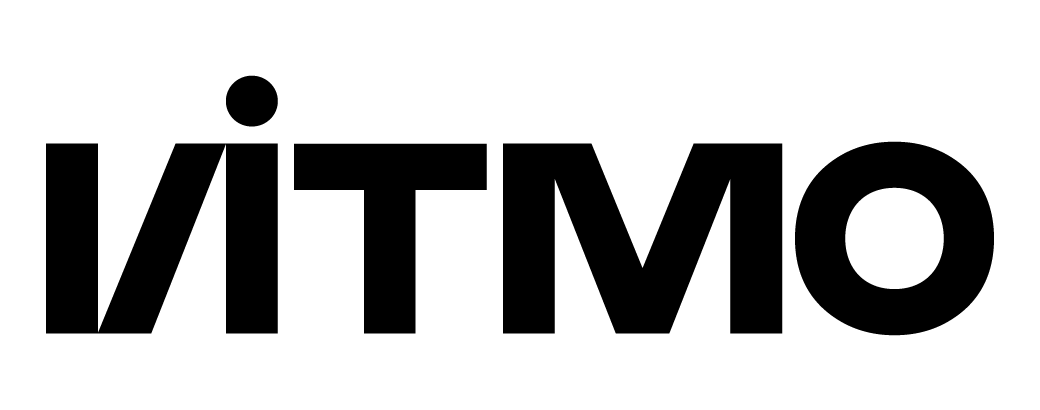
\includegraphics[scale=0.2]{../../lib/img/itmo.png}
\end{center}
\vspace{4cm}


\begin{center}
  \large \textbf{Вариант \textnumero 32}\\
  \textbf{Лабораторная работа \textnumero 1}\\
  по дисциплине\\
  \textbf{Информатика}
\end{center}

\vspace*{\fill}

\begin{flushright}
  Выполнил Студент группы P3115\\
  \textbf{Владимир Мацюк}\\
  Преподаватель: \\
  \textbf{Малышева Татьяна Алексеевна}\\
\end{flushright}

\vspace{1cm}

\begin{center}
  г. Санкт-Петербург\\
  2022г.
\end{center}

\newpage

\lstset{
  inputencoding=utf8,
  frame=single,
  language=Java,
  breaklines=true,
  numbers=left,
  postbreak=\mbox{\textcolor{red}{$\hookrightarrow$}\space},
  extendedchars=false,
  showspaces=false,
  showstringspaces=false,
  basicstyle=\footnotesize\ttfamily,
  identifierstyle=\bf\ttfamily\color[HTML]{2a72de},
  commentstyle=\color[rgb]{0.133,0.545,0.133},
  stringstyle=\color[rgb]{0.133,0.545,0.133},
  keywordstyle=\color[HTML]{5804cf}
}

\section*{Текст задания}

\begin{enumerate}
  \item $ 64073_{10}       = ?_{7}$
        $$ \begin{tabular}{cc}
            64073 div 7 = 9153 & 64073 mod 7 = 2 \\
            9153 div 7 = 1307  & 9153 mod 7 = 4  \\
            1307 div 7 = 186   & 1307 mod 7 = 5  \\
            186 div 7 = 26     & 186 mod 7 = 4   \\
            26 div 7 = 3       & 26 mod 7 = 5    \\
            3 div 7 = 0        & 3 mod 7 = 3     \\
          \end{tabular}
          \Rightarrow
          64073_{10} = 354542_{7}
        $$
  \item $ 31234_{5}        = ?_{10}$
        $$ 3\cdot5^4 + 1\cdot5^3 + 2\cdot5^2 + 3\cdot5^1 + 4\cdot5^0 =
          2069_{10}
        $$
  \item $ B0524_{13}       = ?_{7}$
        $$ B\cdot13^4 + 0\cdot13^3 + 5\cdot13^2 + 2\cdot13^1 + 4\cdot13^0 = 315046_{10}
        $$ $$
          \begin{tabular}{cc}
            315046 div 7 = 45006 & 315046 mod 7 = 4 \\
            45006 div 7 = 6429   & 45006 mod 7 = 3  \\
            6429 div 7 = 918     & 6429 mod 7 = 3   \\
            918 div 7 = 131      & 918 mod 7 = 1    \\
            131 div 7 = 18       & 131 mod 7 = 5    \\
            18 div 7 = 2         & 18 mod 7 = 4     \\
            2 div 7 = 0          & 2 mod 7 = 2      \\
          \end{tabular}
          \Rightarrow
          B0524_{13} = 315046_{10} = 2451334_{7}
        $$
  \item $ 95,73_{10}       = ?_{2}$
        $$   \begin{tabular}{cc}
            95 div 2 = 47 & 95 mod 2 = 1 \\
            47 div 2 = 23 & 47 mod 2 = 1 \\
            23 div 2 = 11 & 23 mod 2 = 1 \\
            11 div 2 = 5  & 11 mod 2 = 1 \\
            5 div 2 = 2   & 5 mod 2 = 1  \\
            2 div 2 = 1   & 2 mod 2 = 0  \\
            1 div 2 = 0   & 1 mod 2 = 1  \\
          \end{tabular}
          \Rightarrow
          95{10} = 1011111_{2}
        $$
        $$
          \begin{tabular}{c}
            0.73·2 = 1.46 \\
            0.46·2 = 0.92 \\
            0.92·2 = 1.84 \\
            0.84·2 = 1.68 \\
            0.68·2 = 1.36 \\
            0.36·2 = 0.72 \\
            0.72·2 = 1.44 \\
            0.44·2 = 0.88 \\
            0.88·2 = 1.76 \\
            0.76·2 = 1.52 \\
            0.52·2 = 1.04 \\
            0.04·2 = 0.08 \\
            0.08·2 = 0.16 \\
            0.16·2 = 0.32 \\
            0.32·2 = 0.64 \\
            0.64·2 = 1.28 \\
            0.28·2 = 0.56 \\
            0.56·2 = 1.12 \\
            0.12·2 = 0.24 \\
            0.24·2 = 0.48 \\
            0.48·2 = 0.96 \\
            0.96·2 = 1.92 \\
          \end{tabular}
          \Rightarrow
          0,73{10} = 0,10(11101011100001010001)_{2}
        $$ $$
          95,73_{10} = 1011111,10(11101011100001010001)_{2}
        $$
  \item $ EA,D9_{16}       = ?_{2}$
        $$
          EA,D9_{16}       = 1110\:1010,1101\:1001_{2}
          \;\;\;\;\;\;\;\\
          \begin{tabular}{cc}
            Hex & Bin  \\
            \hline
            0   & 0000 \\
            \hline
            1   & 0001 \\
            \hline
            2   & 0010 \\
            \hline
            3   & 0011 \\
            \hline
            4   & 0100 \\
            \hline
            5   & 0101 \\
            \hline
            6   & 0110 \\
            \hline
            7   & 0111 \\
            \hline
            8   & 1000 \\
            \hline
            9   & 1001 \\
            \hline
            A   & 1010 \\
            \hline
            B   & 1011 \\
            \hline
            C   & 1100 \\
            \hline
            D   & 1101 \\
            \hline
            E   & 1110 \\
            \hline
            F   & 1111 \\
            \hline
          \end{tabular}
        $$
  \item $ 41,17_{8}        = ?_{2}$
        $$
          41,17_{8}       = 100\:001,001\:111_{2}
          \;\;\;\;\;\;\;\\
          \begin{tabular}{cc}
            Oct & Bin \\
            \hline
            0   & 000 \\
            \hline
            1   & 001 \\
            \hline
            2   & 010 \\
            \hline
            3   & 011 \\
            \hline
            4   & 100 \\
            \hline
            5   & 101 \\
            \hline
            6   & 110 \\
            \hline
            7   & 111 \\
            \hline
          \end{tabular}
        $$
  \item $ 0,100001_{2}     = ?_{16}$
        $$
          0,100001_{2} = 0,1000\:0100_{2} = 0,84_{16}
          \;\;\;\;\;\;\;\\
          \begin{tabular}{cc}
            Hex & Bin  \\
            \hline
            0   & 0000 \\
            \hline
            1   & 0001 \\
            \hline
            2   & 0010 \\
            \hline
            3   & 0011 \\
            \hline
            4   & 0100 \\
            \hline
            5   & 0101 \\
            \hline
            6   & 0110 \\
            \hline
            7   & 0111 \\
            \hline
            8   & 1000 \\
            \hline
            9   & 1001 \\
            \hline
            A   & 1010 \\
            \hline
            B   & 1011 \\
            \hline
            C   & 1100 \\
            \hline
            D   & 1101 \\
            \hline
            E   & 1110 \\
            \hline
            F   & 1111 \\
            \hline
          \end{tabular}
        $$
  \item $ 0,000001_{2}     = ?_{10}$
        $$  0,000001_{2} = 1\cdot2^{-6} = 0.015625_{10} $$
  \item $ 45,19_{16}       = ?_{10}$
        $$  45,19_{16} =
          4\cdot16^{1} + 5\cdot16^{0} + 1\cdot16^{-1} + 9\cdot16^{-2}  =
          69,09765625_{10} $$
  \item $ 232_{10}         = ?_{Fact}$
        $$
          \begin{tabular}{cc}
            232 div 2 = 116 & 232 mod 2 = 0 \\
            116 div 3 = 38  & 116 mod 3 = 2 \\
            38 div 4 = 9    & 38 mod 4 = 2  \\
            9 div 5 = 1     & 9 mod 5 = 4   \\
            1 div 6 = 0     & 1 mod 6 = 1   \\
          \end{tabular}
          \Rightarrow
          232_{10} = 14220_{Fact}
        $$
  \item $ 1001001_{Fib}    = ?_{10}$
        $$
          1001001_{Fib} = Fib(7) + Fib(4) + Fib(1) = 21 + 5 + 1 = 27_{10}
          \;\;\;\;\;\;\;\\
          \begin{tabular}{cc}
            i & Fib(i) \\
            \hline
            1 & 1      \\
            \hline
            2 & 2      \\
            \hline
            3 & 3      \\
            \hline
            4 & 5      \\
            \hline
            5 & 8      \\
            \hline
            6 & 13     \\
            \hline
            7 & 21     \\
            \hline
          \end{tabular}
        $$
  \item $ 1000000010_{Fib} = ?_{10}$
        $$
          1000000010_{Fib} = Fib(10) + Fib(2) = 89 + 2 = 91_{10}
          \;\;\;\;\;\;\;\\
          \begin{tabular}{cc}
            i  & Fib(i) \\
            \hline
            1  & 1      \\
            \hline
            2  & 2      \\
            \hline
            3  & 3      \\
            \hline
            4  & 5      \\
            \hline
            5  & 8      \\
            \hline
            6  & 13     \\
            \hline
            7  & 21     \\
            \hline
            8  & 34     \\
            \hline
            9  & 55     \\
            \hline
            10 & 89     \\
            \hline
          \end{tabular} $$
  \item $ 1786_{-10} = ?_{10}$
        $$  1786_{-10} = 1\cdot(-10)^3 + 7\cdot(-10)^2 + 8\cdot(-10)^1 + 6\cdot(-10)^0 =
          -374_{10}
        $$

\end{enumerate}

\section*{Вывод}
Я освежил свои знания о системах счисления и выполнил переводы чисел между ними.
\end{document}
